% Options for packages loaded elsewhere
\PassOptionsToPackage{unicode}{hyperref}
\PassOptionsToPackage{hyphens}{url}
%
\documentclass[
]{article}
\usepackage{amsmath,amssymb}
\usepackage{lmodern}
\usepackage{iftex}
\ifPDFTeX
  \usepackage[T1]{fontenc}
  \usepackage[utf8]{inputenc}
  \usepackage{textcomp} % provide euro and other symbols
\else % if luatex or xetex
  \usepackage{unicode-math}
  \defaultfontfeatures{Scale=MatchLowercase}
  \defaultfontfeatures[\rmfamily]{Ligatures=TeX,Scale=1}
\fi
% Use upquote if available, for straight quotes in verbatim environments
\IfFileExists{upquote.sty}{\usepackage{upquote}}{}
\IfFileExists{microtype.sty}{% use microtype if available
  \usepackage[]{microtype}
  \UseMicrotypeSet[protrusion]{basicmath} % disable protrusion for tt fonts
}{}
\makeatletter
\@ifundefined{KOMAClassName}{% if non-KOMA class
  \IfFileExists{parskip.sty}{%
    \usepackage{parskip}
  }{% else
    \setlength{\parindent}{0pt}
    \setlength{\parskip}{6pt plus 2pt minus 1pt}}
}{% if KOMA class
  \KOMAoptions{parskip=half}}
\makeatother
\usepackage{xcolor}
\usepackage[margin=1in]{geometry}
\usepackage{color}
\usepackage{fancyvrb}
\newcommand{\VerbBar}{|}
\newcommand{\VERB}{\Verb[commandchars=\\\{\}]}
\DefineVerbatimEnvironment{Highlighting}{Verbatim}{commandchars=\\\{\}}
% Add ',fontsize=\small' for more characters per line
\usepackage{framed}
\definecolor{shadecolor}{RGB}{248,248,248}
\newenvironment{Shaded}{\begin{snugshade}}{\end{snugshade}}
\newcommand{\AlertTok}[1]{\textcolor[rgb]{0.94,0.16,0.16}{#1}}
\newcommand{\AnnotationTok}[1]{\textcolor[rgb]{0.56,0.35,0.01}{\textbf{\textit{#1}}}}
\newcommand{\AttributeTok}[1]{\textcolor[rgb]{0.77,0.63,0.00}{#1}}
\newcommand{\BaseNTok}[1]{\textcolor[rgb]{0.00,0.00,0.81}{#1}}
\newcommand{\BuiltInTok}[1]{#1}
\newcommand{\CharTok}[1]{\textcolor[rgb]{0.31,0.60,0.02}{#1}}
\newcommand{\CommentTok}[1]{\textcolor[rgb]{0.56,0.35,0.01}{\textit{#1}}}
\newcommand{\CommentVarTok}[1]{\textcolor[rgb]{0.56,0.35,0.01}{\textbf{\textit{#1}}}}
\newcommand{\ConstantTok}[1]{\textcolor[rgb]{0.00,0.00,0.00}{#1}}
\newcommand{\ControlFlowTok}[1]{\textcolor[rgb]{0.13,0.29,0.53}{\textbf{#1}}}
\newcommand{\DataTypeTok}[1]{\textcolor[rgb]{0.13,0.29,0.53}{#1}}
\newcommand{\DecValTok}[1]{\textcolor[rgb]{0.00,0.00,0.81}{#1}}
\newcommand{\DocumentationTok}[1]{\textcolor[rgb]{0.56,0.35,0.01}{\textbf{\textit{#1}}}}
\newcommand{\ErrorTok}[1]{\textcolor[rgb]{0.64,0.00,0.00}{\textbf{#1}}}
\newcommand{\ExtensionTok}[1]{#1}
\newcommand{\FloatTok}[1]{\textcolor[rgb]{0.00,0.00,0.81}{#1}}
\newcommand{\FunctionTok}[1]{\textcolor[rgb]{0.00,0.00,0.00}{#1}}
\newcommand{\ImportTok}[1]{#1}
\newcommand{\InformationTok}[1]{\textcolor[rgb]{0.56,0.35,0.01}{\textbf{\textit{#1}}}}
\newcommand{\KeywordTok}[1]{\textcolor[rgb]{0.13,0.29,0.53}{\textbf{#1}}}
\newcommand{\NormalTok}[1]{#1}
\newcommand{\OperatorTok}[1]{\textcolor[rgb]{0.81,0.36,0.00}{\textbf{#1}}}
\newcommand{\OtherTok}[1]{\textcolor[rgb]{0.56,0.35,0.01}{#1}}
\newcommand{\PreprocessorTok}[1]{\textcolor[rgb]{0.56,0.35,0.01}{\textit{#1}}}
\newcommand{\RegionMarkerTok}[1]{#1}
\newcommand{\SpecialCharTok}[1]{\textcolor[rgb]{0.00,0.00,0.00}{#1}}
\newcommand{\SpecialStringTok}[1]{\textcolor[rgb]{0.31,0.60,0.02}{#1}}
\newcommand{\StringTok}[1]{\textcolor[rgb]{0.31,0.60,0.02}{#1}}
\newcommand{\VariableTok}[1]{\textcolor[rgb]{0.00,0.00,0.00}{#1}}
\newcommand{\VerbatimStringTok}[1]{\textcolor[rgb]{0.31,0.60,0.02}{#1}}
\newcommand{\WarningTok}[1]{\textcolor[rgb]{0.56,0.35,0.01}{\textbf{\textit{#1}}}}
\usepackage{graphicx}
\makeatletter
\def\maxwidth{\ifdim\Gin@nat@width>\linewidth\linewidth\else\Gin@nat@width\fi}
\def\maxheight{\ifdim\Gin@nat@height>\textheight\textheight\else\Gin@nat@height\fi}
\makeatother
% Scale images if necessary, so that they will not overflow the page
% margins by default, and it is still possible to overwrite the defaults
% using explicit options in \includegraphics[width, height, ...]{}
\setkeys{Gin}{width=\maxwidth,height=\maxheight,keepaspectratio}
% Set default figure placement to htbp
\makeatletter
\def\fps@figure{htbp}
\makeatother
\setlength{\emergencystretch}{3em} % prevent overfull lines
\providecommand{\tightlist}{%
  \setlength{\itemsep}{0pt}\setlength{\parskip}{0pt}}
\setcounter{secnumdepth}{-\maxdimen} % remove section numbering
\usepackage{booktabs}
\usepackage{longtable}
\usepackage{array}
\usepackage{multirow}
\usepackage{wrapfig}
\usepackage{float}
\usepackage{colortbl}
\usepackage{pdflscape}
\usepackage{tabu}
\usepackage{threeparttable}
\usepackage{threeparttablex}
\usepackage[normalem]{ulem}
\usepackage{makecell}
\usepackage{xcolor}
\ifLuaTeX
  \usepackage{selnolig}  % disable illegal ligatures
\fi
\IfFileExists{bookmark.sty}{\usepackage{bookmark}}{\usepackage{hyperref}}
\IfFileExists{xurl.sty}{\usepackage{xurl}}{} % add URL line breaks if available
\urlstyle{same} % disable monospaced font for URLs
\hypersetup{
  pdftitle={Accompanying Paper Code},
  hidelinks,
  pdfcreator={LaTeX via pandoc}}

\title{Accompanying Paper Code}
\author{}
\date{\vspace{-2.5em}}

\begin{document}
\maketitle

This vignette is a companion to the paper `The maximally selected
likelihood ratio test in random coefficient models.' The code to build
all figures in that paper are presented. Discussions on these figures
are conducted in the paper and are not addressed in this data
supplement.

The stationary region was built using the following code.

\begin{Shaded}
\begin{Highlighting}[]
\FunctionTok{set.seed}\NormalTok{(}\DecValTok{12345}\NormalTok{)}
\NormalTok{data\_sr }\OtherTok{\textless{}{-}} \FunctionTok{simulateStationaryRegion}\NormalTok{(}\AttributeTok{nSims =} \DecValTok{10000000}\NormalTok{, }\AttributeTok{silent=}\NormalTok{T)}
\end{Highlighting}
\end{Shaded}

The results of that code includes the following figure.

\begin{Shaded}
\begin{Highlighting}[]
\NormalTok{data\_sr[[}\DecValTok{3}\NormalTok{]]}
\end{Highlighting}
\end{Shaded}

\begin{figure}
\centering
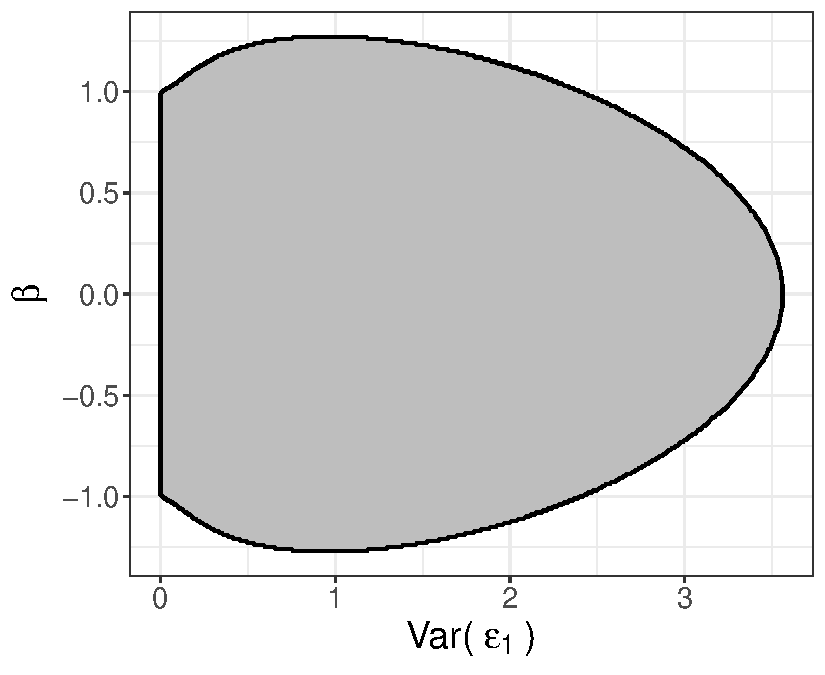
\includegraphics{paperCode_files/figure-latex/plotStationaryRegion-1.pdf}
\caption{Simulation stationary region using Gaussian error based on
\(E\log |\beta + \epsilon_{0,1} |\)}
\end{figure}

The empirical rejection frequencies under the null case was generated
using the following code.

\begin{Shaded}
\begin{Highlighting}[]
\NormalTok{data\_er }\OtherTok{\textless{}{-}} \FunctionTok{simulationTable\_NC}\NormalTok{(}\AttributeTok{betas =} \FunctionTok{c}\NormalTok{(}\FloatTok{0.5}\NormalTok{,}\FloatTok{0.75}\NormalTok{,}\DecValTok{1}\NormalTok{,}\FloatTok{1.05}\NormalTok{), }
                              \AttributeTok{varProbRates =} \FunctionTok{c}\NormalTok{(}\FloatTok{0.5}\NormalTok{, }\FloatTok{0.5}\NormalTok{),}
                              \AttributeTok{nSims=}\DecValTok{500}\NormalTok{, }\AttributeTok{iterations =} \FunctionTok{c}\NormalTok{(}\DecValTok{100}\NormalTok{, }\DecValTok{200}\NormalTok{, }\DecValTok{400}\NormalTok{, }\DecValTok{800}\NormalTok{), }
                              \AttributeTok{burnin =} \DecValTok{1000}\NormalTok{, }\AttributeTok{lowerEst=}\FunctionTok{c}\NormalTok{(}\SpecialCharTok{{-}}\ConstantTok{Inf}\NormalTok{,}\DecValTok{0}\NormalTok{,}\DecValTok{10}\SpecialCharTok{\^{}{-}}\DecValTok{8}\NormalTok{,}\SpecialCharTok{{-}}\ConstantTok{Inf}\NormalTok{), }
                              \AttributeTok{upperEst=}\FunctionTok{c}\NormalTok{(}\ConstantTok{Inf}\NormalTok{,}\ConstantTok{Inf}\NormalTok{,}\ConstantTok{Inf}\NormalTok{,}\ConstantTok{Inf}\NormalTok{), }\AttributeTok{alpha =} \FloatTok{0.05}\NormalTok{,}
                              \AttributeTok{errorTypes =} \FunctionTok{c}\NormalTok{(}\StringTok{\textquotesingle{}Normal\textquotesingle{}}\NormalTok{,}\StringTok{\textquotesingle{}Bernoulli\textquotesingle{}}\NormalTok{,}\StringTok{\textquotesingle{}Exponential\textquotesingle{}}\NormalTok{),}
                              \AttributeTok{CPLoc=}\FloatTok{0.5}\NormalTok{, }\AttributeTok{seed=}\DecValTok{1234}\NormalTok{,}\AttributeTok{trimAmt=}\DecValTok{10}\NormalTok{)}
\end{Highlighting}
\end{Shaded}

The results of that code is the following data.

\begin{Shaded}
\begin{Highlighting}[]
\NormalTok{data\_er}\SpecialCharTok{$}\NormalTok{errType }\OtherTok{\textless{}{-}} \FunctionTok{ifelse}\NormalTok{(data\_er}\SpecialCharTok{$}\NormalTok{errType}\SpecialCharTok{==}\StringTok{\textquotesingle{}Normal\textquotesingle{}}\NormalTok{,}\StringTok{\textquotesingle{}N\textquotesingle{}}\NormalTok{,}
                          \FunctionTok{ifelse}\NormalTok{(data\_er}\SpecialCharTok{$}\NormalTok{errType}\SpecialCharTok{==}\StringTok{\textquotesingle{}Bernoulli\textquotesingle{}}\NormalTok{,}\StringTok{\textquotesingle{}B\textquotesingle{}}\NormalTok{,}\StringTok{\textquotesingle{}E\textquotesingle{}}\NormalTok{))}
\NormalTok{tmp }\OtherTok{\textless{}{-}}\NormalTok{ data\_er }\SpecialCharTok{\%\textgreater{}\%}
\NormalTok{  dplyr}\SpecialCharTok{::}\FunctionTok{select}\NormalTok{(}\SpecialCharTok{{-}}\FunctionTok{c}\NormalTok{(Lower,Upper)) }\SpecialCharTok{\%\textgreater{}\%}
  \FunctionTok{pivot\_wider}\NormalTok{(}\AttributeTok{names\_from =} \FunctionTok{c}\NormalTok{(iters,errType), }\AttributeTok{values\_from =}\NormalTok{ Estim)}

\FunctionTok{kable}\NormalTok{(tmp[,}\SpecialCharTok{!}\NormalTok{(}\FunctionTok{colnames}\NormalTok{(tmp)}\SpecialCharTok{\%in\%}\FunctionTok{c}\NormalTok{(}\StringTok{\textquotesingle{}beta\textquotesingle{}}\NormalTok{))], }\AttributeTok{booktabs =} \ConstantTok{TRUE}\NormalTok{) }\SpecialCharTok{\%\textgreater{}\%}
  \FunctionTok{pack\_rows}\NormalTok{(}\AttributeTok{index =} \FunctionTok{table}\NormalTok{(tmp}\SpecialCharTok{$}\NormalTok{beta))}
\end{Highlighting}
\end{Shaded}

\begin{tabular}{lrrrrrrrrrrrr}
\toprule
type & 100\_N & 200\_N & 400\_N & 800\_N & 100\_B & 200\_B & 400\_B & 800\_B & 100\_E & 200\_E & 400\_E & 800\_E\\
\midrule
\addlinespace[0.3em]
\multicolumn{13}{l}{\textbf{0.5}}\\
\hspace{1em}MLE & 0.002 & 0.012 & 0.004 & 0.010 & 0.002 & 0.006 & 0.006 & 0.004 & 0.006 & 0.010 & 0.028 & 0.016\\
\hspace{1em}Vost & 0.026 & 0.046 & 0.024 & 0.032 & 0.032 & 0.032 & 0.034 & 0.028 & 0.028 & 0.026 & 0.042 & 0.052\\
\hspace{1em}WLS & 0.004 & 0.012 & 0.002 & 0.018 & 0.012 & 0.012 & 0.012 & 0.010 & 0.004 & 0.006 & 0.014 & 0.016\\
\addlinespace[0.3em]
\multicolumn{13}{l}{\textbf{0.75}}\\
\hspace{1em}MLE & 0.002 & 0.010 & 0.002 & 0.010 & 0.010 & 0.006 & 0.004 & 0.004 & 0.004 & 0.008 & 0.022 & 0.026\\
\hspace{1em}Vost & 0.030 & 0.028 & 0.028 & 0.036 & 0.044 & 0.024 & 0.032 & 0.026 & 0.026 & 0.024 & 0.048 & 0.052\\
\hspace{1em}WLS & 0.020 & 0.032 & 0.026 & 0.034 & 0.034 & 0.024 & 0.056 & 0.040 & 0.006 & 0.004 & 0.018 & 0.024\\
\addlinespace[0.3em]
\multicolumn{13}{l}{\textbf{1}}\\
\hspace{1em}MLE & 0.008 & 0.010 & 0.002 & 0.006 & 0.006 & 0.010 & 0.008 & 0.012 & 0.006 & 0.008 & 0.016 & 0.020\\
\hspace{1em}Vost & 0.022 & 0.040 & 0.032 & 0.036 & 0.048 & 0.032 & 0.036 & 0.038 & 0.030 & 0.036 & 0.054 & 0.040\\
\hspace{1em}WLS & 0.030 & 0.054 & 0.058 & 0.058 & 0.076 & 0.098 & 0.138 & 0.142 & 0.002 & 0.004 & 0.018 & 0.016\\
\addlinespace[0.3em]
\multicolumn{13}{l}{\textbf{1.05}}\\
\hspace{1em}MLE & 0.002 & 0.016 & 0.012 & 0.012 & 0.010 & 0.010 & 0.008 & 0.008 & 0.004 & 0.010 & 0.020 & 0.024\\
\hspace{1em}Vost & 0.024 & 0.052 & 0.032 & 0.044 & 0.046 & 0.038 & 0.038 & 0.036 & 0.028 & 0.036 & 0.058 & 0.048\\
\hspace{1em}WLS & 0.026 & 0.078 & 0.058 & 0.066 & 0.066 & 0.090 & 0.136 & 0.150 & 0.004 & 0.006 & 0.014 & 0.016\\
\bottomrule
\end{tabular}

The power curves were built using the following code.

\begin{Shaded}
\begin{Highlighting}[]
\NormalTok{tmp }\OtherTok{\textless{}{-}} \FunctionTok{c}\NormalTok{(}\DecValTok{1}\NormalTok{, }\FloatTok{0.9}\NormalTok{,}\FloatTok{0.75}\NormalTok{, }\FunctionTok{seq}\NormalTok{(}\FloatTok{0.6}\NormalTok{,}\FloatTok{0.3}\NormalTok{,}\SpecialCharTok{{-}}\FloatTok{0.1}\NormalTok{),}\FloatTok{0.25}\NormalTok{,}\FloatTok{0.1}\NormalTok{)}
\NormalTok{U4seq }\OtherTok{\textless{}{-}} \FunctionTok{c}\NormalTok{(tmp, }\DecValTok{0}\NormalTok{, }\FunctionTok{rev}\NormalTok{(}\SpecialCharTok{{-}}\NormalTok{tmp))}
\FunctionTok{set.seed}\NormalTok{(}\DecValTok{1234}\NormalTok{)}
\NormalTok{pc1 }\OtherTok{\textless{}{-}} \FunctionTok{simulatePowerCurve}\NormalTok{(}\AttributeTok{Us3 =} \FunctionTok{c}\NormalTok{(}\DecValTok{0}\NormalTok{, }\FloatTok{0.5}\NormalTok{, }\FloatTok{0.5}\NormalTok{), }\AttributeTok{U4s =}\NormalTok{ U4seq,}
                     \AttributeTok{nSims =} \DecValTok{500}\NormalTok{, }\AttributeTok{lowerEst =} \FunctionTok{c}\NormalTok{(}\SpecialCharTok{{-}}\ConstantTok{Inf}\NormalTok{,}\DecValTok{0}\NormalTok{,}\DecValTok{10}\SpecialCharTok{\^{}{-}}\DecValTok{8}\NormalTok{,}\SpecialCharTok{{-}}\ConstantTok{Inf}\NormalTok{), }
                     \AttributeTok{upperEst =} \FunctionTok{rep}\NormalTok{(}\ConstantTok{Inf}\NormalTok{,}\DecValTok{4}\NormalTok{), }\AttributeTok{alpha =} \FloatTok{0.05}\NormalTok{,}
                     \AttributeTok{burnin =} \DecValTok{1000}\NormalTok{, }\AttributeTok{k =} \FloatTok{0.5} \SpecialCharTok{*} \DecValTok{400}\NormalTok{, }\AttributeTok{N =} \DecValTok{400}\NormalTok{, }
                     \AttributeTok{errorType =} \StringTok{\textquotesingle{}Normal\textquotesingle{}}\NormalTok{, }\AttributeTok{trimAmt=}\DecValTok{10}\NormalTok{,}
                     \AttributeTok{silent=}\NormalTok{T)}

\FunctionTok{set.seed}\NormalTok{(}\DecValTok{1234}\NormalTok{)}
\NormalTok{pc2 }\OtherTok{\textless{}{-}} \FunctionTok{simulatePowerCurve}\NormalTok{(}\AttributeTok{Us3 =} \FunctionTok{c}\NormalTok{(}\DecValTok{0}\NormalTok{, }\FloatTok{0.5}\NormalTok{, }\FloatTok{0.5}\NormalTok{), }\AttributeTok{U4s =}\NormalTok{ U4seq,}
                     \AttributeTok{nSims =} \DecValTok{500}\NormalTok{, }\AttributeTok{lowerEst =} \FunctionTok{c}\NormalTok{(}\SpecialCharTok{{-}}\ConstantTok{Inf}\NormalTok{,}\DecValTok{0}\NormalTok{,}\DecValTok{10}\SpecialCharTok{\^{}{-}}\DecValTok{8}\NormalTok{,}\SpecialCharTok{{-}}\ConstantTok{Inf}\NormalTok{), }
                     \AttributeTok{upperEst =} \FunctionTok{rep}\NormalTok{(}\ConstantTok{Inf}\NormalTok{,}\DecValTok{4}\NormalTok{), }\AttributeTok{alpha =} \FloatTok{0.05}\NormalTok{,}
                     \AttributeTok{burnin =} \DecValTok{1000}\NormalTok{, }\AttributeTok{k =} \FloatTok{0.9} \SpecialCharTok{*} \DecValTok{400}\NormalTok{, }\AttributeTok{N =} \DecValTok{400}\NormalTok{, }
                     \AttributeTok{errorType =} \StringTok{\textquotesingle{}Normal\textquotesingle{}}\NormalTok{, }\AttributeTok{trimAmt=}\DecValTok{10}\NormalTok{,}
                     \AttributeTok{silent=}\NormalTok{T)}

\NormalTok{U4seq }\OtherTok{\textless{}{-}} \FunctionTok{c}\NormalTok{(}\FloatTok{1.05}\NormalTok{,}\FunctionTok{seq}\NormalTok{(}\DecValTok{1}\NormalTok{,}\FloatTok{0.6}\NormalTok{,}\SpecialCharTok{{-}}\FloatTok{0.1}\NormalTok{), }\FloatTok{0.5}\NormalTok{, }\FunctionTok{seq}\NormalTok{(}\FloatTok{0.4}\NormalTok{,}\DecValTok{0}\NormalTok{,}\SpecialCharTok{{-}}\FloatTok{0.1}\NormalTok{),}\SpecialCharTok{{-}}\FloatTok{0.05}\NormalTok{)}
\FunctionTok{set.seed}\NormalTok{(}\DecValTok{1234}\NormalTok{)}
\NormalTok{pc3 }\OtherTok{\textless{}{-}} \FunctionTok{simulatePowerCurve}\NormalTok{(}\AttributeTok{Us3 =} \FunctionTok{c}\NormalTok{(}\FloatTok{0.5}\NormalTok{, }\FloatTok{0.5}\NormalTok{, }\FloatTok{0.5}\NormalTok{), }\AttributeTok{U4s =}\NormalTok{ U4seq,}
                     \AttributeTok{nSims =} \DecValTok{500}\NormalTok{, }\AttributeTok{lowerEst =} \FunctionTok{c}\NormalTok{(}\SpecialCharTok{{-}}\ConstantTok{Inf}\NormalTok{,}\DecValTok{0}\NormalTok{,}\DecValTok{10}\SpecialCharTok{\^{}{-}}\DecValTok{8}\NormalTok{,}\SpecialCharTok{{-}}\ConstantTok{Inf}\NormalTok{), }
                     \AttributeTok{upperEst =} \FunctionTok{rep}\NormalTok{(}\ConstantTok{Inf}\NormalTok{,}\DecValTok{4}\NormalTok{), }\AttributeTok{alpha =} \FloatTok{0.05}\NormalTok{,}
                     \AttributeTok{burnin =} \DecValTok{1000}\NormalTok{, }\AttributeTok{k =} \FloatTok{0.5} \SpecialCharTok{*} \DecValTok{400}\NormalTok{, }\AttributeTok{N =} \DecValTok{400}\NormalTok{, }
                     \AttributeTok{errorType =} \StringTok{\textquotesingle{}Normal\textquotesingle{}}\NormalTok{, }\AttributeTok{trimAmt=}\DecValTok{10}\NormalTok{,}
                     \AttributeTok{silent=}\NormalTok{T)}
\FunctionTok{set.seed}\NormalTok{(}\DecValTok{1234}\NormalTok{)}
\NormalTok{pc4 }\OtherTok{\textless{}{-}} \FunctionTok{simulatePowerCurve}\NormalTok{(}\AttributeTok{Us3 =} \FunctionTok{c}\NormalTok{(}\FloatTok{0.5}\NormalTok{, }\FloatTok{0.5}\NormalTok{, }\FloatTok{0.5}\NormalTok{), }\AttributeTok{U4s =}\NormalTok{ U4seq,}
                     \AttributeTok{nSims =} \DecValTok{500}\NormalTok{, }\AttributeTok{lowerEst =} \FunctionTok{c}\NormalTok{(}\SpecialCharTok{{-}}\ConstantTok{Inf}\NormalTok{,}\DecValTok{0}\NormalTok{,}\DecValTok{10}\SpecialCharTok{\^{}{-}}\DecValTok{8}\NormalTok{,}\SpecialCharTok{{-}}\ConstantTok{Inf}\NormalTok{), }
                     \AttributeTok{upperEst =} \FunctionTok{rep}\NormalTok{(}\ConstantTok{Inf}\NormalTok{,}\DecValTok{4}\NormalTok{), }\AttributeTok{alpha =} \FloatTok{0.05}\NormalTok{,}
                     \AttributeTok{burnin =} \DecValTok{1000}\NormalTok{, }\AttributeTok{k =} \FloatTok{0.5} \SpecialCharTok{*} \DecValTok{400}\NormalTok{, }\AttributeTok{N =} \DecValTok{400}\NormalTok{,}
                     \AttributeTok{errorType =} \StringTok{\textquotesingle{}Bernoulli\textquotesingle{}}\NormalTok{, }\AttributeTok{trimAmt=}\DecValTok{10}\NormalTok{,}
                     \AttributeTok{silent=}\NormalTok{T)}
\end{Highlighting}
\end{Shaded}

The resulting power figures are as follows (See the paper for details on
each of the figures).

\begin{Shaded}
\begin{Highlighting}[]
\NormalTok{pc1[[}\DecValTok{1}\NormalTok{]]}
\end{Highlighting}
\end{Shaded}

\begin{figure}
\centering
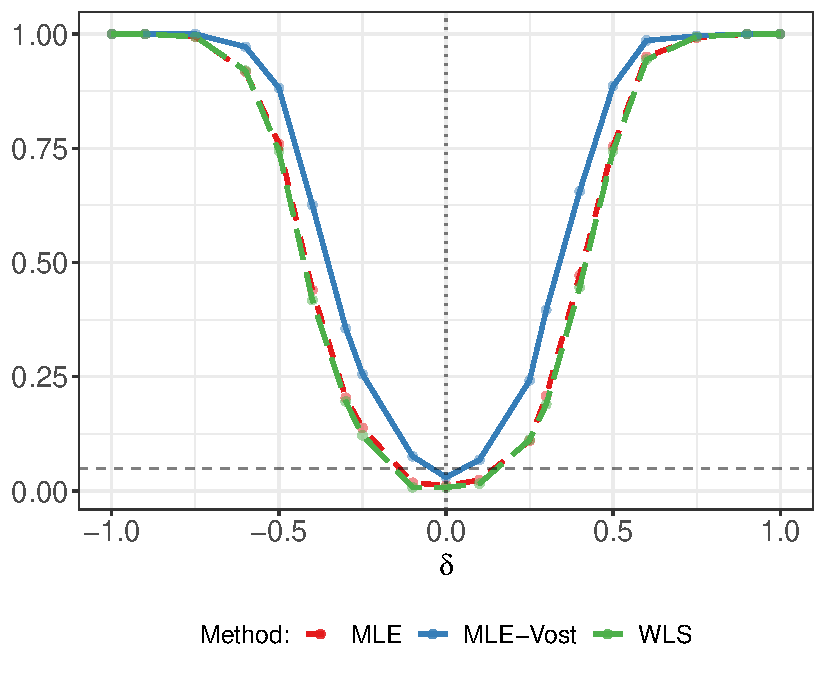
\includegraphics{paperCode_files/figure-latex/plotPowerCurves-1.pdf}
\caption{Power curves as a function of the change in RCA coefficient.}
\end{figure}

\begin{Shaded}
\begin{Highlighting}[]
\NormalTok{pc2[[}\DecValTok{1}\NormalTok{]]}
\end{Highlighting}
\end{Shaded}

\begin{figure}
\centering
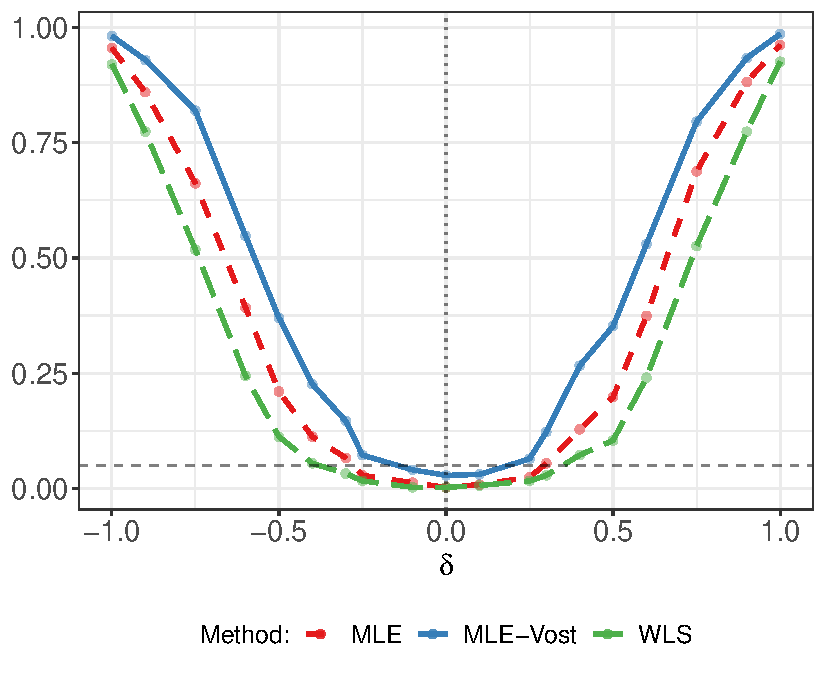
\includegraphics{paperCode_files/figure-latex/plotPowerCurves-2.pdf}
\caption{Power curves as a function of the change in RCA coefficient.}
\end{figure}

\begin{Shaded}
\begin{Highlighting}[]
\NormalTok{pc3[[}\DecValTok{1}\NormalTok{]]}
\end{Highlighting}
\end{Shaded}

\begin{figure}
\centering
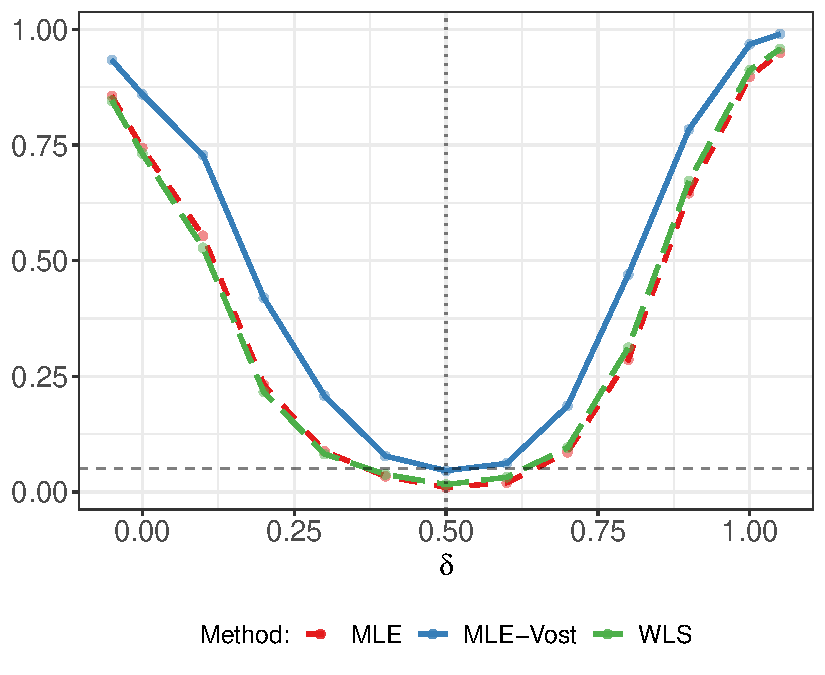
\includegraphics{paperCode_files/figure-latex/plotPowerCurves-3.pdf}
\caption{Power curves as a function of the change in RCA coefficient.}
\end{figure}

\begin{Shaded}
\begin{Highlighting}[]
\NormalTok{pc4[[}\DecValTok{1}\NormalTok{]]}
\end{Highlighting}
\end{Shaded}

\begin{figure}
\centering
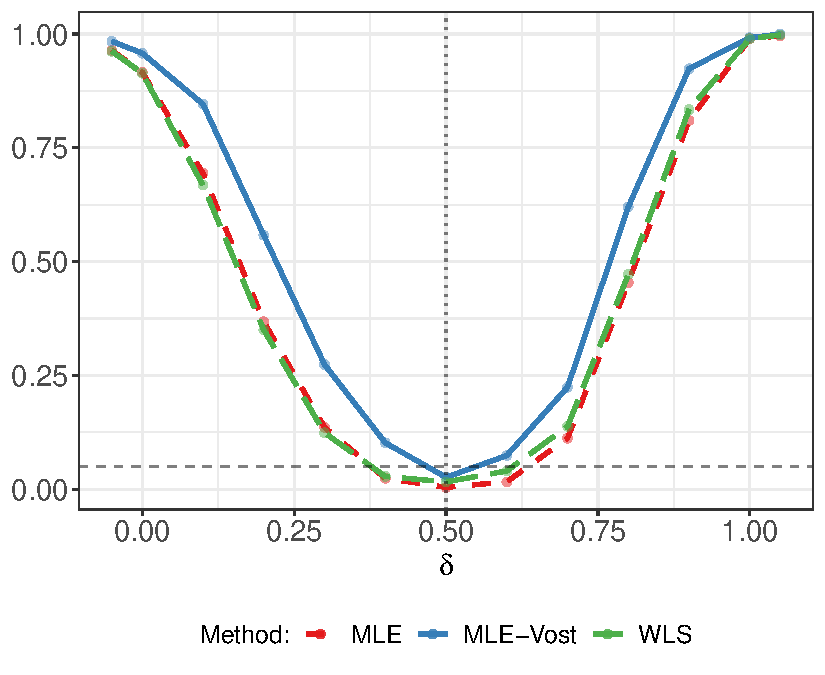
\includegraphics{paperCode_files/figure-latex/plotPowerCurves-4.pdf}
\caption{Power curves as a function of the change in RCA coefficient.}
\end{figure}

The US housing figures were built using the following code.

\begin{Shaded}
\begin{Highlighting}[]
\NormalTok{housingDataList }\OtherTok{\textless{}{-}} \FunctionTok{list}\NormalTok{()}
\ControlFlowTok{for}\NormalTok{(city }\ControlFlowTok{in} \FunctionTok{c}\NormalTok{(}\StringTok{\textquotesingle{}Boston\textquotesingle{}}\NormalTok{,}\StringTok{\textquotesingle{}LosAngeles\textquotesingle{}}\NormalTok{))\{}
  
  \DocumentationTok{\#\# Load data}
\NormalTok{  data }\OtherTok{\textless{}{-}}\NormalTok{ housing[housing}\SpecialCharTok{$}\NormalTok{city}\SpecialCharTok{==}\NormalTok{city,}\FunctionTok{c}\NormalTok{(}\DecValTok{2}\NormalTok{,}\DecValTok{3}\NormalTok{)]}
\NormalTok{  data }\OtherTok{\textless{}{-}}\NormalTok{ data[}\FunctionTok{order}\NormalTok{(data}\SpecialCharTok{$}\NormalTok{date),]}
  
  \DocumentationTok{\#\# Detect CP}
  \FunctionTok{set.seed}\NormalTok{(}\DecValTok{12345}\NormalTok{)}
\NormalTok{  result\_Vost }\OtherTok{\textless{}{-}} \FunctionTok{binarySegmentationCPDetection}\NormalTok{(}\AttributeTok{fullData=}\NormalTok{data, }
                                       \AttributeTok{method=}\StringTok{\textquotesingle{}Vostrikova\textquotesingle{}}\NormalTok{,}
                                       \AttributeTok{lower=}\FunctionTok{c}\NormalTok{(}\SpecialCharTok{{-}}\ConstantTok{Inf}\NormalTok{, }\DecValTok{0}\NormalTok{, }\DecValTok{10}\SpecialCharTok{\^{}{-}}\DecValTok{8}\NormalTok{, }\SpecialCharTok{{-}}\ConstantTok{Inf}\NormalTok{),}
                                       \AttributeTok{upper=}\FunctionTok{c}\NormalTok{(}\ConstantTok{Inf}\NormalTok{, }\ConstantTok{Inf}\NormalTok{, }\ConstantTok{Inf}\NormalTok{, }\ConstantTok{Inf}\NormalTok{),}
                                       \AttributeTok{alpha=}\FloatTok{0.05}\NormalTok{, }\AttributeTok{nStart=}\ConstantTok{NA}\NormalTok{, }\AttributeTok{nEnd=}\ConstantTok{NA}\NormalTok{,}
                                       \AttributeTok{trimAmt =} \DecValTok{10}\NormalTok{, }\AttributeTok{silent =}\NormalTok{ T )}
  
\NormalTok{  data\_plot }\OtherTok{\textless{}{-}} \FunctionTok{renderStackedPlot}\NormalTok{(}\AttributeTok{trueData =}\NormalTok{ data, }
                     \AttributeTok{parCPData =}\NormalTok{ result\_Vost[,}\FunctionTok{c}\NormalTok{(}\DecValTok{1}\SpecialCharTok{:}\DecValTok{2}\NormalTok{,}\DecValTok{7}\SpecialCharTok{:}\DecValTok{10}\NormalTok{)],}
                     \AttributeTok{title =} \ConstantTok{NULL}\NormalTok{,}
                     \AttributeTok{subtitle =} \ConstantTok{NULL}\NormalTok{,}
                     \AttributeTok{varPlots =} \ConstantTok{FALSE}\NormalTok{)}
  
  \DocumentationTok{\#\# Save data}
\NormalTok{  housingDataList }\OtherTok{\textless{}{-}} \FunctionTok{append}\NormalTok{(housingDataList, }\FunctionTok{list}\NormalTok{(}\FunctionTok{list}\NormalTok{(result\_Vost,data\_plot)))}
\NormalTok{\}}
\end{Highlighting}
\end{Shaded}

The results were as follows.

\begin{Shaded}
\begin{Highlighting}[]
\NormalTok{housingDataList[[}\DecValTok{1}\NormalTok{]][[}\DecValTok{2}\NormalTok{]]}
\end{Highlighting}
\end{Shaded}

\begin{figure}
\centering
\includegraphics{paperCode_files/figure-latex/plotHousingData_Boston-1.pdf}
\caption{Daily US housing price indices in Boston.}
\end{figure}

\begin{Shaded}
\begin{Highlighting}[]
\NormalTok{housingDataList[[}\DecValTok{2}\NormalTok{]][[}\DecValTok{2}\NormalTok{]]}
\end{Highlighting}
\end{Shaded}

\begin{figure}
\centering
\includegraphics{paperCode_files/figure-latex/plotHousingData_LA-1.pdf}
\caption{Daily US housing price indices in Los Angeles.}
\end{figure}

The UK covid-19 figures were built using the subsequent code.

\begin{Shaded}
\begin{Highlighting}[]
\NormalTok{UKCovidList }\OtherTok{\textless{}{-}} \FunctionTok{list}\NormalTok{()}
\ControlFlowTok{for}\NormalTok{(nation }\ControlFlowTok{in} \FunctionTok{c}\NormalTok{(}\StringTok{\textquotesingle{}England\textquotesingle{}}\NormalTok{,}\StringTok{\textquotesingle{}Northern Ireland\textquotesingle{}}\NormalTok{,}\StringTok{\textquotesingle{}Scotland\textquotesingle{}}\NormalTok{,}\StringTok{\textquotesingle{}Wales\textquotesingle{}}\NormalTok{))\{}
  
  \DocumentationTok{\#\# Load data}
\NormalTok{  data }\OtherTok{\textless{}{-}}\NormalTok{ UKcovid[UKcovid}\SpecialCharTok{$}\NormalTok{nation}\SpecialCharTok{==}\NormalTok{nation,}\FunctionTok{c}\NormalTok{(}\DecValTok{2}\NormalTok{,}\DecValTok{3}\NormalTok{)]}
\NormalTok{  data }\OtherTok{\textless{}{-}}\NormalTok{ data[}\FunctionTok{order}\NormalTok{(data}\SpecialCharTok{$}\NormalTok{date),]}
  
  \DocumentationTok{\#\# Detect CP}
  \FunctionTok{set.seed}\NormalTok{(}\DecValTok{12345}\NormalTok{)}
\NormalTok{  result\_Vost }\OtherTok{\textless{}{-}} \FunctionTok{binarySegmentationCPDetection}\NormalTok{(}\AttributeTok{fullData=}\NormalTok{data, }
                                       \AttributeTok{method=}\StringTok{\textquotesingle{}Vostrikova\textquotesingle{}}\NormalTok{,}
                                       \AttributeTok{lower=}\FunctionTok{c}\NormalTok{(}\SpecialCharTok{{-}}\ConstantTok{Inf}\NormalTok{, }\DecValTok{0}\NormalTok{, }\DecValTok{10}\SpecialCharTok{\^{}{-}}\DecValTok{8}\NormalTok{, }\SpecialCharTok{{-}}\ConstantTok{Inf}\NormalTok{),}
                                       \AttributeTok{upper=}\FunctionTok{c}\NormalTok{(}\ConstantTok{Inf}\NormalTok{, }\ConstantTok{Inf}\NormalTok{, }\ConstantTok{Inf}\NormalTok{, }\ConstantTok{Inf}\NormalTok{),}
                                       \AttributeTok{alpha=}\FloatTok{0.05}\NormalTok{,}
                                       \AttributeTok{trimAmt =} \DecValTok{10}\NormalTok{, }\AttributeTok{silent =}\NormalTok{ T )}
\NormalTok{  data\_plot }\OtherTok{\textless{}{-}} \FunctionTok{renderStackedPlot}\NormalTok{(}\AttributeTok{trueData =}\NormalTok{ data, }
                     \AttributeTok{parCPData =}\NormalTok{ result\_Vost[,}\FunctionTok{c}\NormalTok{(}\DecValTok{1}\SpecialCharTok{:}\DecValTok{2}\NormalTok{,}\DecValTok{7}\SpecialCharTok{:}\DecValTok{10}\NormalTok{)],}
                     \AttributeTok{title =} \ConstantTok{NULL}\NormalTok{,}
                     \AttributeTok{subtitle =} \ConstantTok{NULL}\NormalTok{,}
                     \AttributeTok{varPlots =} \ConstantTok{FALSE}\NormalTok{)}
  
  \DocumentationTok{\#\# Save data}
\NormalTok{  UKCovidList }\OtherTok{\textless{}{-}} \FunctionTok{append}\NormalTok{(UKCovidList, }\FunctionTok{list}\NormalTok{(}\FunctionTok{list}\NormalTok{(result\_Vost,data\_plot)))}
\NormalTok{\}}
\end{Highlighting}
\end{Shaded}

With plots produced as follows.

\begin{Shaded}
\begin{Highlighting}[]
\NormalTok{UKCovidList[[}\DecValTok{1}\NormalTok{]][[}\DecValTok{2}\NormalTok{]]}
\end{Highlighting}
\end{Shaded}

\begin{figure}
\centering
\includegraphics{paperCode_files/figure-latex/plotUKCovidData_England-1.pdf}
\caption{\label{fig:UKCovid}Daily Covid-19 patients hospitalised in
England.}
\end{figure}

\begin{Shaded}
\begin{Highlighting}[]
\NormalTok{UKCovidList[[}\DecValTok{2}\NormalTok{]][[}\DecValTok{2}\NormalTok{]]}
\end{Highlighting}
\end{Shaded}

\begin{figure}
\centering
\includegraphics{paperCode_files/figure-latex/plotUKCovidData_NIreland-1.pdf}
\caption{\label{fig:UKCovid}Daily Covid-19 patients hospitalised in
Northern Ireland.}
\end{figure}

\begin{Shaded}
\begin{Highlighting}[]
\NormalTok{UKCovidList[[}\DecValTok{3}\NormalTok{]][[}\DecValTok{2}\NormalTok{]]}
\end{Highlighting}
\end{Shaded}

\begin{figure}
\centering
\includegraphics{paperCode_files/figure-latex/plotUKCovidData_Scotland-1.pdf}
\caption{\label{fig:UKCovid}Daily Covid-19 patients hospitalised in
Scotland.}
\end{figure}

\begin{Shaded}
\begin{Highlighting}[]
\NormalTok{UKCovidList[[}\DecValTok{4}\NormalTok{]][[}\DecValTok{2}\NormalTok{]]}
\end{Highlighting}
\end{Shaded}

\begin{figure}
\centering
\includegraphics{paperCode_files/figure-latex/plotUKCovidData_Wales-1.pdf}
\caption{\label{fig:UKCovid}Daily Covid-19 patients hospitalised in
Wales.}
\end{figure}

\end{document}
